% !TEX program = latexmk
% Compile example:
% latexmk -pdfdvi -latex='uplatex -synctex=1 -interaction=nonstopmode -file-line-error' -dvipdf='dvipdfmx %O -o %D %S' spilled_energy_lecture_beamer.tex

\documentclass[dvipdfmx,uplatex,unicode,9pt,aspectratio=169]{beamer}

% Japanese / dvipdfmx support
\usepackage{bxdpx-beamer}
\usepackage{pxjahyper}
\usepackage{minijs}

% Math / tables / graphics
\usepackage{amsmath,amssymb,mathtools}
\usepackage{booktabs,array,multirow}
\usepackage{bm}
\usepackage{graphicx}
\usepackage{xcolor}
\newcommand{\redbox}[1]{%
  {\color{red}\boxed{\color{black}#1}}%
}

\usepackage{physics2}
\usephysicsmodule{ab}

\usepackage{tikz}
\usetikzlibrary{arrows.meta,positioning,calc}
\usepackage{url}
\graphicspath{{figures/}}

\usepackage{tcolorbox}

% タイトルなし・beamer block 風の青い枠
\newtcolorbox{notitleblock}{
  colback=structure.fg!8,
  colframe=structure.fg!75!black,
  boxrule=0.6pt,
  arc=2pt,
  left=7pt,
  right=7pt,
  top=6pt,
  bottom=6pt,
  before skip=7pt,
  after skip=7pt
}

% -------- Theme --------
\usetheme{default}
\usefonttheme{professionalfonts}
\beamertemplatenavigationsymbolsempty

\definecolor{Navy}{HTML}{0B1F33}
\definecolor{Blue}{HTML}{2563EB}
\definecolor{Cyan}{HTML}{0891B2}
\definecolor{Green}{HTML}{10B981}
\definecolor{Red}{HTML}{EF4444}
\definecolor{Amber}{HTML}{F59E0B}
\definecolor{GrayText}{HTML}{475467}
\definecolor{PaleBlue}{HTML}{EFF6FF}
\definecolor{PaleGreen}{HTML}{ECFDF5}
\definecolor{PaleRed}{HTML}{FEF2F2}
\definecolor{PaleAmber}{HTML}{FFFBEB}
\definecolor{LightGray}{HTML}{F2F4F7}

\setbeamercolor{normal text}{fg=Navy,bg=white}
\setbeamercolor{frametitle}{fg=white,bg=Navy}
\setbeamercolor{title}{fg=white,bg=Navy}
\setbeamercolor{subtitle}{fg=white,bg=Navy}
\setbeamercolor{block title}{fg=white,bg=Blue}
\setbeamercolor{block body}{fg=Navy,bg=PaleBlue}
\setbeamercolor{alerted text}{fg=Red}
\setbeamercolor{example text}{fg=Green}
\setbeamercolor{itemize item}{fg=Blue}
\setbeamercolor{itemize subitem}{fg=Cyan}
\setbeamerfont{frametitle}{size=\Large,series=\bfseries}
\setbeamerfont{title}{size=\huge,series=\bfseries}
\setbeamerfont{subtitle}{size=\large}
\setbeamerfont{author}{size=\small}
\setbeamerfont{date}{size=\small}

\setbeamertemplate{footline}{%
  \leavevmode%
  \hbox{%
  \begin{beamercolorbox}[wd=.78\paperwidth,ht=2.7ex,dp=1.1ex,leftskip=1.2em]{author in head/foot}%
    \color{GrayText}\scriptsize Spilled Energy in LLMs
  \end{beamercolorbox}%
  \begin{beamercolorbox}[wd=.22\paperwidth,ht=2.7ex,dp=1.1ex,rightskip=1.2em plus1fil]{date in head/foot}%
    \hfill\color{GrayText}\scriptsize \insertframenumber/\inserttotalframenumber
  \end{beamercolorbox}}%
}

\newcommand{\key}[1]{\textcolor{Blue}{\textbf{#1}}}
\newcommand{\good}[1]{\textcolor{Green}{\textbf{#1}}}
\newcommand{\bad}[1]{\textcolor{Red}{\textbf{#1}}}
\newcommand{\notegray}[1]{\textcolor{GrayText}{\footnotesize #1}}
\newcommand{\tok}[1]{\texttt{#1}}
\newcommand{\source}[1]{\vfill{\tiny\color{GrayText}出典: #1}}
\newcommand{\metric}[1]{\textbf{\textcolor{Blue}{#1}}}
\newcommand{\DeltaE}{\Delta E_{\theta}}
\newcommand{\El}{E^{\ell}_{\theta}}
\newcommand{\Em}{E^{m}_{\theta}}
\newcommand{\LSE}{\operatorname{LSE}}

\title{Spilled Energy in Large Language Models}
\subtitle{LLMのハルシネーション検出を「エネルギーのズレ」として読む}
\author{
発表者：山口 海 \\[1ex]
{\small 論文著者：Adrian R. Minut, Hazem Dewidar, Iacopo Masi}\\[0.5ex]
\notegray{\small arXiv:2602.18671v4 / ICLR 2026 conference paper}
}

\date{
論文紹介 \\[0.5ex]
\today
}

\begin{document}

% 1
\begin{frame}[plain]
  \begin{beamercolorbox}[wd=\paperwidth,ht=\paperheight,center,sep=0pt]{title}
    \vspace{1.75cm}
    {\usebeamerfont{title}\inserttitle\par}
    \vspace{0.5cm}
    {\usebeamerfont{subtitle}\insertsubtitle\par}
    \vspace{1.0cm}
    {\usebeamerfont{author}\insertauthor\par}
    \vfill
    {\scriptsize 論文: \url{https://arxiv.org/abs/2602.18671}\quad Code: \url{https://github.com/OmnAI-Lab/spilled-energy/}}
    \vspace{0.6cm}
  \end{beamercolorbox}

\end{frame}

% 3
\begin{frame}{論文の狙い: 追加学習なしで誤答検出}
\begin{columns}[T,onlytextwidth]
\begin{column}{0.32\linewidth}
\begin{block}{問い}
LLMの回答が\bad{誤答/ハルシネーション}かどうかを、外部検索や追加学習なしで検出できるか？
\end{block}
\end{column}
\begin{column}{0.32\linewidth}
\begin{block}{着眼点}
最終softmaxを\key{Energy-Based Model}として解釈し、連続する生成ステップ間でそろうはずのエネルギーを比較する。
\end{block}
\end{column}
\begin{column}{0.32\linewidth}
\begin{block}{結論}
出力logitだけから計算する\key{spilled energy}が、複数タスク・複数LLMで誤答検出に有効。
\end{block}
\end{column}
\end{columns}
\centering
\includegraphics[width=0.8\linewidth]{figures/fig5.png}
\vspace{0.6em}
\begin{center}
\fcolorbox{Blue}{PaleBlue}{\parbox{0.88\linewidth}{\centering
\textbf{核心:} 「生成された答えトークンの自信」だけではなく、\textbf{そのトークンを含むprefixが次の時刻でどれだけ整合的な分布を作るか}を見る。
}}
\end{center}
\source{Minut et al., \textit{Spilled Energy in Large Language Models}, Abstract and Sec. 1.}
\end{frame}

% 2
\begin{frame}{LLM内部の流れ: textから次トークン確率まで}
\small
\begin{center}
\resizebox{0.96\linewidth}{!}{%
\begin{tikzpicture}[
  box/.style={draw=Navy, rounded corners, thick, align=center, minimum height=0.93cm, inner sep=4pt, font=\small, fill=white},
  arrow/.style={-{Stealth[length=2.4mm]}, very thick, draw=Navy}
]
\node[box, minimum width=3.0cm] (text) {入力text\\\tok{The capital of Italy is Rome}};
\node[box, minimum width=2.65cm, right=0.55cm of text] (tok) {tokenizer\\token列 $x_1,\ldots,x_6$};
\node[box, minimum width=2.75cm, right=0.55cm of tok] (ids) {token IDs\\$[1023,845,319,2048,374,912]$};
\node[box, minimum width=2.85cm, right=0.55cm of ids] (oh) {one-hot行列\\$X_{\mathrm{oh}}\in\mathbb{R}^{N\times V}$};
\node[box, minimum width=3.0cm, below=0.82cm of oh] (emb) {埋め込み\\$H^{(0)}=X_{\mathrm{oh}}W_{\mathrm{emb}}$};
\node[box, minimum width=2.9cm, left=0.55cm of emb] (trf) {Transformer\\因果maskで文脈処理};
\node[box, minimum width=2.9cm, left=0.55cm of trf] (logit) {logitベクトル\\$\theta(x_{i:1})\in\mathbb{R}^{V}$};
\node[box, minimum width=2.9cm, left=0.55cm of logit] (softmax) {softmax\\次トークン確率};
\draw[arrow] (text) -- (tok);
\draw[arrow] (tok) -- (ids);
\draw[arrow] (ids) -- (oh);
\draw[arrow] (oh) -- (emb);
\draw[arrow] (emb) -- (trf);
\draw[arrow] (trf) -- (logit);
\draw[arrow] (logit) -- (softmax);
\end{tikzpicture}%
}
\end{center}
\vspace{0.5em}
\begin{columns}[T,onlytextwidth]
\begin{column}{0.5\linewidth}
  \centering
\begin{tabular}{c c c}
\toprule
位置 & token $x_i$ & $\mathrm{id}(x_i)$ \\
\midrule
1 & \tok{The} & 1023 \\
2 & \tok{capital} & 845 \\
3 & \tok{of} & 319 \\
4 & \tok{Italy} & 2048 \\
5 & \tok{is} & 374 \\
6 & \tok{Rome} & 912 \\
\bottomrule
\end{tabular}
\fcolorbox{Blue}{PaleBlue}{\parbox{0.93\linewidth}{

LLM全体を抽象的に$\theta:\mathbb{R}^{N\times V}\to\mathbb{R}^{V}$という関数として表す。
$\theta(x_{i:1})[k]$は文脈$x_{i:1}$の次に語彙ID $k$ が出るlogitである。
}}
\end{column}
\begin{column}{0.5\linewidth}
  \centering
  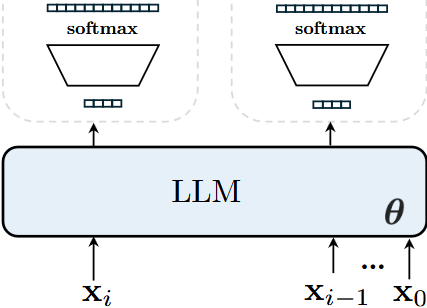
\includegraphics[width=0.65\linewidth]{fig7.png}
\end{column}
\end{columns}
\end{frame}

% 4
\begin{frame}{IDから埋め込み、logit、softmaxへ}
\small
\begin{columns}[T,onlytextwidth]
\begin{column}{0.49\linewidth}
\begin{block}{1. token ID $\rightarrow$ one-hot}
語彙サイズを $V$ とすると、各token IDはone-hot行に変換できる。
\[
X_{\mathrm{oh}}=
\begin{bmatrix}
\bm e_{1023}^{\top}\\
\bm e_{845}^{\top}\\
\bm e_{319}^{\top}\\
\bm e_{2048}^{\top}\\
\bm e_{374}^{\top}\\
\bm e_{912}^{\top}
\end{bmatrix}
\in\mathbb{R}^{6\times V}
\]
\end{block}
\begin{block}{2. one-hot $\rightarrow$ 埋め込み}
\[
W_{\mathrm{emb}}\in\mathbb{R}^{V\times d},\quad
H^{(0)}=X_{\mathrm{oh}}W_{\mathrm{emb}}\in\mathbb{R}^{N\times d}.
\]
one-hotで、埋め込み行列の該当行を取り出している。
\end{block}
\end{column}
\begin{column}{0.49\linewidth}
\begin{block}{3. Transformer $\rightarrow$ hidden state}
因果maskにより、位置 $i$ のhidden stateはprefixだけを見る。
\[
H=\mathrm{Transformer}(H^{(0)}),\quad h_i=f_\theta(x_{i:1}).
\]
\end{block}
\begin{block}{4. hidden state $\rightarrow$ logit $\rightarrow$ softmax}
\[
\theta(x_{i:1})=h_iW_{\mathrm{out}}+b\in\mathbb{R}^{V}
\]
\[
p_\theta(x_{i+1}=k\mid x_{i:1})
=\frac{\exp(\theta(x_{i:1})[k])}
{\sum_{j=1}^{V}\exp(\theta(x_{i:1})[j])}.
\]
\end{block}
\end{column}
\end{columns}
\end{frame}

% 5
\begin{frame}{例: \tok{Rome} を生成するステップ}
\small
\begin{columns}[T,onlytextwidth]
\begin{column}{0.49\linewidth}
\begin{block}{prefixと次トークン}
\[
\underbrace{(\tok{The},\tok{capital},\tok{of},\tok{Italy},\tok{is})}_{x_{5:1}\;\text{に対応}}
\rightarrow
\underbrace{\tok{Rome}}_{x_6}
\]
モデルはprefix $x_{5:1}$ から語彙全体のlogit
\[
\theta(x_{5:1})\in\mathbb{R}^{V}
\]
を出す。
\end{block}
\begin{block}{\tok{Rome} のlogit}
\[
\mathrm{id}(\tok{Rome})=912
\]
\[
\theta(x_{5:1})[\mathrm{id}(x_6)]
=\theta(x_{5:1})[912]
\]
が、\tok{Rome} を選ぶためのsoftmax前スコア。
\end{block}
\end{column}
\begin{column}{0.49\linewidth}
\begin{block}{softmax後の確率}
\[
p_\theta(x_6=\tok{Rome}\mid x_{5:1})
=\frac{\exp(\theta(x_{5:1})[912])}
{\sum_{k=1}^{V}\exp(\theta(x_{5:1})[k])}.
\]
\end{block}
\begin{block}{spilled energyへの接続}
\tok{Rome} を検出対象にすると、後で見る量は
\[
\DeltaE(x_{6:1})
=\LSE(\theta(x_{6:1}))-\theta(x_{5:1})[\mathrm{id}(x_6)].
\]
つまり、\tok{Rome} を出したlogitと、\tok{Rome} を含めた次stepの語彙全体logsumexpを照合する。
\end{block}
\end{column}
\end{columns}
\end{frame}



% 7
\begin{frame}{LLMは次の1トークンの予想を繰り返す}
\begin{block}{トークン列}
$x_{i:1}=(x_i,x_{i-1},\ldots,x_1)$ と書く。つまり$x_{i:1}$ は「1番目から $i$ 番目までの文脈」を表す順序付き系列である。
\end{block}
\begin{block}{自己回帰モデル}
\begin{align}
  p(x_{i:1}) &= p_\theta(x_1)\prod_{t=2}^{i}p_\theta(x_t\mid x_{t-1:1}) \label{eq:autoregressive} \\
 &= p_\theta(x_1)p_\theta(x_2\mid x_1)p_\theta(x_3\mid x_{2:1})\cdots p_\theta(x_t\mid x_{t-1:1}) \cdots p_\theta(x_i\mid x_{i-1:1})
\end{align}
\end{block}
ステップ$t$の条件付き確率は、直前の文脈$x_{t-1:1}$ から次トークン $x_t$ を予測する。
\begin{equation}
  p_\theta(x_t\mid x_{t-1:1}) = \frac{p_\theta(x_{t:1})}{p_\theta(x_{t-1:1})} \label{eq:conditional_probability}
\end{equation}
\end{frame}

% 8
\begin{frame}{Step 1:中間項のキャンセル}
\eqref{eq:conditional_probability} を\eqref{eq:autoregressive}に代入すると、
\begin{align*}
  p(x_{i:1}) &= p_\theta(x_1)\prod_{t=2}^{i}\frac{p_\theta(x_{t:1})}{p_\theta(x_{t-1:1})} \\
  &= p_\theta(x_1)p_\theta(x_2\mid x_1)p_\theta(x_3\mid x_{2:1})\cdots p_\theta(x_t\mid x_{t-1:1})
  p_\theta(x_{t+1}\mid x_{t:1})
   \cdots p_\theta(x_i\mid x_{i-1:1}) \\
  &= p_\theta(x_1)\frac{p_\theta(x_{2:1})}{p_\theta(x_1)}\frac{p_\theta(x_{3:1})}{p_\theta(x_{2:1})}\cdots \underbrace{\frac{p_\theta(x_{t:1})}{p_\theta(x_{t-1:1})} }_{\text{ステップ }t} \underbrace{\frac{p_\theta(x_{t+1:1})}{p_\theta(x_{t:1})} }_{\text{ステップ }t+1} \cdots \frac{p_\theta(x_{i:1})}{p_\theta(x_{i-1:1})} \\
  &= p_\theta(x_{i:1}).
\end{align*}
\vspace{-2em}
\begin{columns}[T,onlytextwidth]
\begin{column}{0.48\linewidth}
  \begin{block}{LLM実装上}
    同じ $x_{t:1}$ に関わる量が，
\begin{itemize}
\item 時刻 $t$：$x_t$ を生成したときの\alert{単一logit}
\item 時刻 $t+1$：$x_t$ まで含めた文脈から出す\alert{語彙全体のlog-sum-exp}
\end{itemize}
として測られる。
\end{block}
\end{column}
\begin{column}{0.48\linewidth}
  \centering
  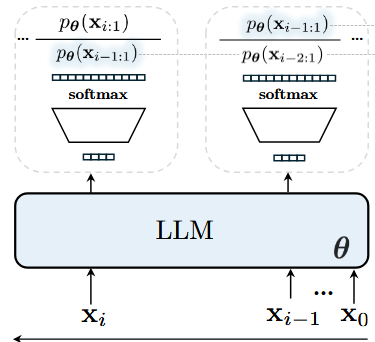
\includegraphics[width=0.65\linewidth]{fig6.png}
\end{column}
\end{columns}
  
\source{Minut et al., Eq. (1)--(2).}
\end{frame}

% 9
\begin{frame}{Step 2: LLMの1-step予測はsoftmax分類器}
LLMの1-step予測は、語彙上のsoftmax分類器である。
\begin{align}
 p_{\theta}(x_i\mid x_{i-1:1})
 =\frac{p_\theta(x_{i:1})}{p_\theta(x_{i-1:1})}
 = \frac{\exp\left(\theta(x_{i-1:1})[\mathrm{id}(x_i)]\right)}
 {\sum_{k=1}^{V}\exp\left(\theta(x_{i-1:1})[k]\right)}.
 \label{eq:softmax}
\end{align}
\begin{columns}[T,onlytextwidth]
\begin{column}{0.48\linewidth}
\begin{block}{分子}
実際に生成されたトークン $x_i$ のlogitだけを読む。
\[
 \theta(x_{i-1:1})[\mathrm{id}(x_i)].
\]
\end{block}
\end{column}
\begin{column}{0.48\linewidth}
\begin{block}{分母}
語彙全体のlogitを合計して正規化項を作る。
\[
 \sum_{k=1}^{V}\exp(\theta(x_{i-1:1})[k]).
\]
\end{block}
\end{column}
\end{columns}
EBMでは、確率を「低エネルギーほど高確率」と読む。
\[
 p_{\theta}(x)=\frac{\exp(-E_\theta(x))}{Z_\theta}.
\]
この見方をsoftmaxに適用すると、LLMの1-step予測は2つのエネルギーに分かれる。
\source{Minut et al., Eq. (3).}
\end{frame}

% 10
\begin{frame}{Step 3: softmax分類器をEBMとして読む}

\begin{columns}[T,onlytextwidth]
\begin{column}{0.48\linewidth}
\begin{block}{logit energy}
\[
 \El(x_{i:1})
 \coloneqq -\theta(x_{i-1:1})[\mathrm{id}(x_i)].
\]
生成されたトークンのlogitを負にしたもの。
\end{block}
\end{column}
\begin{column}{0.48\linewidth}
\begin{block}{marginal energy}
\[
 \Em(x_{i-1:1})
 \coloneqq -\log\sum_{k=1}^{V}\exp(\theta(x_{i-1:1})[k]).
\]
次トークン全候補で周辺化したprefix側のエネルギー。
\end{block}
\end{column}
\end{columns}
この新しく定義した2つのエネルギーを使うと、LLMの1-step予測は
\begin{align}
  p_{\theta}(x_i\mid x_{i-1:1})
  &= \frac{\exp\left(\theta(x_{i-1:1})[\mathrm{id}(x_i)]\right)}
 {\sum_{k=1}^{V}\exp\left(\theta(x_{i-1:1})[k]\right)} = \frac{\exp(-\El(x_{i:1}))}{\exp(-\Em(x_{i-1:1}))} \notag \\
  &= \exp\left\{-\El(x_{i:1})+\Em(x_{i-1:1})\right\}.
  \label{eq:ebm_form}
\end{align}
となり、EBMの形で解釈できる。
\source{Minut et al., Eq. (4)--(7).}
\end{frame}

% 11
\begin{frame}{Step 4: 系列全体の負の対数尤度は、エネルギーの差の和になる}
\eqref{eq:ebm_form} を負の対数尤度にすると、
\begin{align}
 -\log p_\theta(x_i\mid x_{i-1:1})= \El(x_{i:1})-\Em(x_{i-1:1}).
\end{align}
となる。
ここで系列全体に対して負の対数尤度を取ると、各ステップのエネルギーの差の和になる。
\eqref{eq:autoregressive} より、
\begin{align}
 -\log p_\theta(x_{i:1}) &= -\log p_\theta(x_1)\prod_{t=2}^{i}p_\theta(x_t\mid x_{t-1:1}) \notag \\ 
  &= -\log p_\theta(x_1) p_\theta(x_2\mid x_1)p_\theta(x_3\mid x_{2:1})\cdots p_\theta(x_i\mid x_{i-1:1}) \notag \\
  &= -\log p_\theta(x_1) \frac{p_\theta(x_{2:1})}{p_\theta(x_1)}
  \cdots 
  \underbrace{\frac{\redbox{p_\theta(x_{t:1})}}{p_\theta(x_{t-1:1})}}_{\text{ステップ }t}
  \underbrace{\frac{p_\theta(x_{t+1:1})}{\redbox{p_\theta(x_{t:1})}} }_{\text{ステップ }t+1}
  \cdots \frac{p_\theta(x_{i:1})}{p_\theta(x_{i-1:1})} \notag \\
  &= ( \El(x_{1:1})-\Em(x_{0:1})) + \cdots + (\underbrace{\redbox{\El(x_{t:1})}-\Em(x_{t-1:1})}_{\text{ステップ }t}) + (\underbrace{\El(x_{t+1:1})-\redbox{\Em(x_{t:1})}}_{\text{ステップ }t+1}) + \cdots + \El(x_{i:1})-\Em(x_{i-1:1}) \notag \\
  &= \sum_{t=1}^{i} \left\{\El(x_{t:1})-\Em(x_{t-1:1})\right\}.
\end{align}

\end{frame}

% 13
\begin{frame}{Step 5: そのズレを Spilled Energy と呼ぶ}
\begin{block}{定義}
spilled energyは、理論的には同じprefixのエネルギーとして一致してほしいが、実際のLLMでは\textbf{異なる時刻}かつ\textbf{異なるsoftmax成分}から測られる2量の差である。
\end{block}
\vspace{-0.2em}
\begin{equation}
 \DeltaE(x_{i:1}) \coloneqq -\Em(x_{i:1})+\El(x_{i:1})
= \log\sum_{k=1}^{V}\exp(\theta(x_{i:1})[k]) - \theta(x_{i-1:1})[\mathrm{id}(x_i)].
\end{equation}
\vspace{-0.5em}
\begin{columns}[T,onlytextwidth]
\begin{column}{0.49\linewidth}
\begin{block}{timestep $i$: token logit}
\[
\El(x_{i:1})
= -\theta(x_{i-1:1})[\mathrm{id}(x_i)].
\]
\end{block}
\end{column}
\begin{column}{0.49\linewidth}
\begin{block}{timestep $i+1$: logsumexp}
\[
-\Em(x_{i:1})
=\log\sum_{k=1}^{V}\exp(\theta(x_{i:1})[k]).
\]
\end{block}
\end{column}
\end{columns}
\begin{block}{何を比べているか}
\begin{itemize}
\item $\theta(x_{i-1:1})[\mathrm{id}(x_i)]$：$x_i$ を生成した時刻の単一logit．
\item $\log\sum_k\exp\{\theta(x_{i:1})[k]\}$：$x_i$ まで含めた次時刻の語彙全体の正規化項．
\end{itemize}
\end{block}
\source{Minut et al., Definition 4.1 and Eq. (8).}
\end{frame}

% 16
\begin{frame}{具体例: 検出対象を \texttt{Rome} にする}
\footnotesize
\begin{center}
\fcolorbox{Navy}{LightGray}{\parbox{0.93\linewidth}{\centering
出力を単語単位で簡略化: \quad
$x_1=$\texttt{The}, $x_2=$\texttt{caapital}, $x_3=$\texttt{of}, $x_4=$\texttt{Italy}, $x_5=$\texttt{is}, $x_6=$\texttt{Rome}, $x_7=$\texttt{.}
}}
\end{center}
\vspace{0.3em}
\begin{columns}[T,onlytextwidth]
\begin{column}{0.49\linewidth}
\begin{block}{A. 6番目を出すステップ}
\textbf{入力prefix:} \texttt{The caapital of Italy is}
\[
\theta(x_{5:1})[\mathrm{id}(x_6)]
\]
ここでは、$x_6=\texttt{Rome}$ のlogitを読む。
\end{block}
\end{column}
\begin{column}{0.49\linewidth}
\begin{block}{B. 7番目を予測するステップ}
\textbf{入力prefix:} \texttt{The caapital of Italy is Rome}
\[
\LSE(\theta(x_{6:1}))
=\log\sum_k\exp(\theta(x_{6:1})[k])
\]
\texttt{.} のlogit単体ではなく、語彙全体を見る。
\end{block}
\end{column}
\end{columns}
\vspace{0.2em}
\begin{center}
\fcolorbox{Blue}{PaleBlue}{\parbox{0.93\linewidth}{
\[
\DeltaE(x_{6:1})
=\LSE(\theta(x_{6:1}))-\theta(x_{5:1})[\mathrm{id}(x_6)].
\]
\centering
検出対象が\texttt{Rome}なら、\texttt{Rome}を出したlogitと、\texttt{Rome}を含めた次stepの語彙全体logsumexpを照合する。
}}
\includegraphics[width=\linewidth]{fig5.png}
\notegray{緑ほどtruthful、赤ほどhallucinationとして可視化。}
\end{center}
\end{frame}

% 5
\begin{frame}{誤答検出のための比較: 既存手法とSpilled Energy}
\begin{center}
\renewcommand{\arraystretch}{1.25}
\begin{tabular}{p{0.18\linewidth}p{0.35\linewidth}p{0.36\linewidth}}
\toprule
\textbf{方法} & \textbf{見るもの} & \textbf{弱点}\\
\midrule
\metric{logit confidence} & 生成された答えトークンのlogit/確率 & 高確率で誤答を出す「自信過剰」を見逃す。\\
\metric{$p(\mathrm{true})$} & 「この回答は正しいか？」に対するtrueの確率 & 自己評価能力と回答生成能力は一致しない。\\
\metric{probe classifier} & hidden state / activationに訓練した分類器 & タスク・データセット・層・トークン位置に依存しやすい。\\
\metric{spilled energy} & 連続生成ステップのエネルギーのズレ & logitアクセスと答え部分の同定が必要。\\
\bottomrule
\end{tabular}
\end{center}
\vspace{0.4em}
\notegray{論文の狙いは「probeを訓練せず、logit confidenceより深い信号を取る」こと。}
\end{frame}

% 6
\begin{frame}{probe classifier との対比}
\begin{columns}[T,onlytextwidth]
\begin{column}{0.49\linewidth}
\begin{block}{Probe classifier}
\begin{enumerate}
\item 質問と回答をLLMに通す。
\item 特定層・特定位置のhidden stateを取り出す。
\item 小さな分類器を\textbf{正解/誤答ラベル}で訓練する。
\item 新しい回答がhallucinationかを予測する。
\end{enumerate}
\end{block}
\end{column}
\begin{column}{0.49\linewidth}
\begin{block}{Spilled energy}
\begin{enumerate}
\item 質問に対して回答を生成する。
\item 生成時の\textbf{logit列}を保存する。
\item exact answer tokenに限定する。
\item 追加学習なしで $\DeltaE$ を計算する。
\end{enumerate}
\end{block}
\end{column}
\end{columns}
\vspace{0.8em}
\begin{center}
\fcolorbox{Amber}{PaleAmber}{\parbox{0.86\linewidth}{\centering
Probeは\textbf{表現を学習して読む}。Spilled energyは\textbf{softmaxの数理構造を直接読む}。
}}
\end{center}
\source{Minut et al., Sec. 1.}
\end{frame}

% 17
\begin{frame}{実用パイプライン: どこにスコアをかけるか}
\begin{center}
\renewcommand{\arraystretch}{1.25}
\begin{tabular}{p{0.10\linewidth}p{0.72\linewidth}p{0.12\linewidth}}
\toprule
\textbf{Step} & \textbf{処理} & \textbf{出力}\\
\midrule
1 & LLMに質問を入れて回答を生成。生成時のlogitを保存。 & 回答列\\
2 & 回答中の\key{exact answer token}を特定。 & $[u,w]$\\
3 & 各答えトークンで $\Em$ と $\DeltaE$ を計算。 & token score\\
4 & 複数トークンならpooling。論文ではmin poolingが良い傾向。 & answer score\\
5 & 閾値またはランキングで誤答候補を検出。 & warning\\
\bottomrule
\end{tabular}
\end{center}
\vspace{0.6em}
\begin{center}
\fcolorbox{Blue}{PaleBlue}{\parbox{0.90\linewidth}{\centering
ポイント: 文章全体ではなく、\textbf{意味的に答えを担う短いspan}にスコアを絞る。
}}
\end{center}
\source{Minut et al., Sec. 4.2.}
\end{frame}

% 18
\begin{frame}{Exact answer token が重要}
\begin{columns}[T,onlytextwidth]
\begin{column}{0.50\linewidth}
\begin{block}{なぜ必要か}
\begin{itemize}
\item 句読点・文頭語などは次トークン候補が自然に広い。
\item そのためlogsumexpが大きくなり、false positiveが出やすい。
\item 真偽信号は「答えの中身」に集中しやすい。
\end{itemize}
\end{block}
\begin{block}{同定方法}
\begin{itemize}
\item closed-set: 文字列マッチング。
\item open-ended: 補助LLMで短い答えを抽出。
\item 抽出失敗時は再試行またはサンプル除外。
\end{itemize}
\end{block}
\end{column}
\begin{column}{0.47\linewidth}
\centering
\renewcommand{\arraystretch}{1.22}
\begin{tabular}{lcc}
\toprule
\textbf{方法} & \textbf{Pool} & \textbf{Avg. AuROC}\\
\midrule
Logit $\El$ & Max & 56.12\\
Orgad et al. & Mean & 63.67\\
Marginal $\Em$ & Min & 67.23\\
Marginal $\Em$ & Max & 63.34\\
\textbf{Spilled $\DeltaE$} & \textbf{Min} & \textbf{73.32}\\
\bottomrule
\end{tabular}
\vspace{0.6em}
\begin{center}
\fcolorbox{Blue}{PaleBlue}{\parbox{0.90\linewidth}{\centering
exact answerを使うと、Spilled $\DeltaE$ は平均AuROCで約24ポイント改善。
}}
\end{center}
\end{column}
\end{columns}
\source{Minut et al., Table 2 and Sec. 5.2.}
\end{frame}

% 19
\begin{frame}{Pooling: token scoreをanswer scoreにする}
\begin{block}{複数tokenの答え}
答えが複数トークンに分かれるときは、exact answer span $[u,w]$ の各tokenにスコアを計算する。
\[
 \left\{\DeltaE(x_{u:1}),\DeltaE(x_{u+1:1}),\ldots,\DeltaE(x_{w:1})\right\}.
\]
\end{block}
\begin{columns}[T,onlytextwidth]
\begin{column}{0.31\linewidth}
\begin{block}{min pooling}
\[
 \min_{i\in[u,w]}\DeltaE(x_{i:1})
\]
論文で全体的に良い傾向。
\end{block}
\end{column}
\begin{column}{0.31\linewidth}
\begin{block}{max pooling}
\[
 \max_{i\in[u,w]}\DeltaE(x_{i:1})
\]
局所的な大きな異常を拾う。
\end{block}
\end{column}
\begin{column}{0.31\linewidth}
\begin{block}{mean pooling}
\[
 \frac{1}{w-u+1}\sum_{i=u}^{w}\DeltaE(x_{i:1})
\]
span全体の平均を見る。
\end{block}
\end{column}
\end{columns}
\vspace{0.4em}
\begin{center}
\fcolorbox{Amber}{PaleAmber}{\parbox{0.88\linewidth}{\centering
poolingは性能に影響する。論文はmethodごとにpoolingをablationし、平均AuROCで比較している。
}}
\end{center}
\source{Minut et al., Sec. 4.2, Table 2, Appendix B.1.}
\end{frame}

% 21
\begin{frame}{実験1: 合成算術タスクの設計}
\begin{columns}[T,onlytextwidth]
\begin{column}{0.48\linewidth}
\begin{block}{目的}
正解と誤答を制御できる環境で、spilled energyが誤差のある数値回答を分けられるかを確認する。
\end{block}
\begin{block}{問題}
13桁以上の整数加算を生成し、正しい解答と誤った解答を用意する。
\end{block}
\end{column}
\begin{column}{0.48\linewidth}
\begin{block}{誤答の作り方}
正解にランダムなoffsetを加える。
\begin{itemize}
\item Easy: $U(10^3,10^4)$
\item Medium: $U(10^2,10^3)$
\item Hard: $U(1,10)$
\end{itemize}
Hardは数値差が小さく、ぱっと見では plausible。
\end{block}
\begin{block}{モデル}
Llama-3 8B, Qwen-3 8B, Mistral-7B-Instruct v0.3。
\end{block}
\end{column}
\end{columns}
\source{Minut et al., Sec. 5.1.}
\end{frame}

% 22
\begin{frame}{実験1の結果: 誤差が小さくても分離できるか}
\begin{columns}[T,onlytextwidth]
\begin{column}{0.30\linewidth}
\begin{block}{図の読み方}
\begin{itemize}
\item ヒストグラム: correctとincorrectのスコア分布。
\item ROC: しきい値を動かした検出性能。
\item 列が右に行くほど難しい。
\end{itemize}
\end{block}
\begin{block}{観察}
\begin{itemize}
\item 正解は低いspilled energyに寄る。
\item 誤答は高いspilled energyに寄る。
\item Hardでもlogitより強い傾向。
\end{itemize}
\end{block}
\end{column}
\begin{column}{0.67\linewidth}
\centering
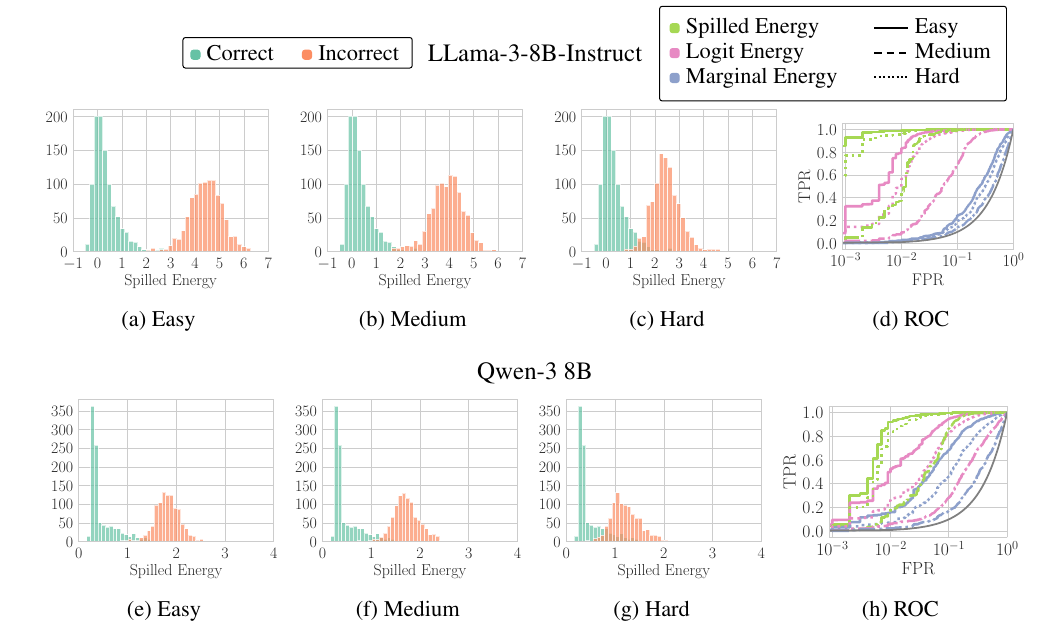
\includegraphics[width=\linewidth]{fig3_synthetic}
\end{column}
\end{columns}
\source{Minut et al., Fig. 3.}
\end{frame}

% 23
\begin{frame}{実験2: 実世界9ベンチマークの設計}
\begin{columns}[T,onlytextwidth]
\begin{column}{0.50\linewidth}
\begin{block}{データセット}
Math, TriviaQA, HotpotQA, Winogrande, Winobias, Movies, MNLI, IMDB, HotpotQA-WC。
\end{block}
\begin{block}{評価したいこと}
\begin{itemize}
\item factual QAだけでなく、推論・分類・バイアス系タスクでも信号が出るか。
\item instruction-tunedとbase modelの両方で機能するか。
\item 追加訓練なしで複数タスクに一般化するか。
\end{itemize}
\end{block}
\end{column}
\begin{column}{0.46\linewidth}
\begin{block}{モデル}
\begin{itemize}
\item LLaMA系: base / instruct
\item Mistral系: base / instruct
\item Gemma系: 1B / 4B instruct
\end{itemize}
\end{block}
\begin{block}{ラベル}
各回答をcorrect / incorrectに分け、検出スコアのAuROCを計算する。
\end{block}
\end{column}
\end{columns}
\source{Minut et al., Sec. 5.2.}
\end{frame}

% 24
\begin{frame}{実世界ベンチマーク: 平均AuROCの要点}
\begin{center}
\renewcommand{\arraystretch}{1.25}
\begin{tabular}{lccccc}
\toprule
\textbf{モデル} & $p(\mathrm{true})$ & \textbf{Probe} & \textbf{Logit} & \textbf{Best Marginal} & \textbf{Spilled $\DeltaE$}\\
\midrule
LLaMA-Instruct & 51.29 & 64.16 & 54.62 & 65.72 & \textbf{73.16}\\
LLaMA base & 54.90 & 62.84 & 56.89 & 59.36 & \textbf{68.69}\\
Mistral-Instruct & 55.88 & 65.56 & 63.44 & 71.12 & \textbf{77.49}\\
Mistral base & 51.36 & 62.11 & 49.51 & \textbf{77.19} & 73.94\\
\bottomrule
\end{tabular}
\end{center}
\vspace{0.7em}
\begin{columns}[T,onlytextwidth]
\begin{column}{0.49\linewidth}
\begin{block}{読み方}
AuROC 50付近はほぼランダム。$p(\mathrm{true})$やlogitは平均的に弱く、タスク依存の揺れが大きい。
\end{block}
\end{column}
\begin{column}{0.49\linewidth}
\begin{block}{結論}
Spilled energyは多くのモデルで平均性能が高い。ただしMistral baseのようにmarginal energyが上回る場合もある。
\end{block}
\end{column}
\end{columns}
\source{Minut et al., Table 1.}
\end{frame}


% 26
\begin{frame}{実験3: Cross-dataset generalization}
\begin{columns}[T,onlytextwidth]
\begin{column}{0.36\linewidth}
\begin{block}{何を調べるか}
Probe classifierをあるデータセットで訓練し、別のデータセットでテストする。
\end{block}
\begin{block}{なぜ重要か}
実際のユーザー入力はタスクが固定されない。訓練データセットに閉じた検出器は、実運用では使いにくい。
\end{block}
\begin{block}{図の見方}
右図(b)の赤い値は、Spilled $\DeltaE$ がprobeより改善している場所。off-diagonalでの改善が重要。
\end{block}
\end{column}
\begin{column}{0.61\linewidth}
\centering
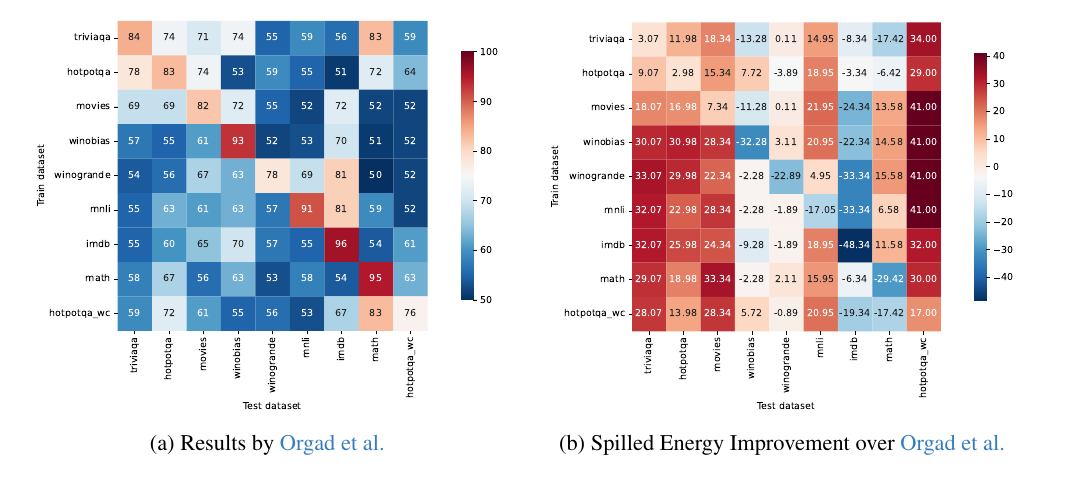
\includegraphics[width=\linewidth]{fig4_cross_dataset}
\end{column}
\end{columns}
\source{Minut et al., Fig. 4 and Sec. 5.2.}
\end{frame}

% 29
\begin{frame}{失敗しやすいケースと限界}
\begin{columns}[T,onlytextwidth]
\begin{column}{0.49\linewidth}
\begin{block}{false positive}
\begin{itemize}
\item 句読点、文頭語、機能語は意味内容が薄い。
\item 次トークン候補が自然に広く、logsumexpが大きくなりやすい。
\item そのため、答えではないtokenで高いspilled energyが出ることがある。
\end{itemize}
\end{block}
\begin{block}{対策}
exact answer tokenに限定する。回答全体に一律でかけると、局所的なfalse positiveが混ざる。
\end{block}
\end{column}
\begin{column}{0.49\linewidth}
\begin{block}{実用上の限界}
\begin{itemize}
\item white-boxなlogitアクセスが必要。
\item APIによっては語彙全体のlogitが取れない。
\item しきい値はモデル・ドメインで校正が必要。
\item 外部事実検証ではないので、真偽の証明にはならない。
\end{itemize}
\end{block}
\begin{center}
\fcolorbox{Navy}{LightGray}{\parbox{0.88\linewidth}{\centering
位置づけ: RAG/外部検証と併用する\textbf{内部不確実性・異常検出スコア}。
}}
\end{center}
\end{column}
\end{columns}
\source{Minut et al., Sec. 5.2, Sec. 6, Appendix D.2.}
\end{frame}

% 30
\begin{frame}{実装チェックリスト}
\begin{columns}[T,onlytextwidth]
\begin{column}{0.48\linewidth}
\begin{block}{必要なデータ}
\begin{itemize}
\item 生成されたtoken ID列。
\item 各stepの語彙全体logit。
\item prompt長と回答token範囲。
\item exact answer span $[u,w]$。
\end{itemize}
\end{block}
\begin{block}{各tokenで計算}
\[
\DeltaE(x_{i:1})
=\LSE(\theta(x_{i:1}))
-\theta(x_{i-1:1})[\mathrm{id}(x_i)].
\]
\end{block}
\end{column}
\begin{column}{0.48\linewidth}
\begin{block}{注意点}
\begin{itemize}
\item tokenizationにより、答え文字列とtoken spanがずれる。
\item 生成時logitと再forward時logitを混同しない。
\item temperatureやlogit processorの影響を確認する。
\item モデルごとにスコア分布を可視化して校正する。
\end{itemize}
\end{block}
\begin{block}{出力}
token-level heatmap、answer-level score、しきい値判定を分けて保存すると解析しやすい。
\end{block}
\end{column}
\end{columns}
\end{frame}

% 31
\begin{frame}{この論文の貢献を3つに整理}
\begin{columns}[T,onlytextwidth]
\begin{column}{0.32\linewidth}
\begin{block}{数理的貢献}
最終softmaxをEBMとして読み、chain ruleから本来整合するはずの2つのエネルギーを取り出した。
\end{block}
\end{column}
\begin{column}{0.32\linewidth}
\begin{block}{方法的貢献}
probe classifierや追加訓練なしで、logit列からtoken-localなhallucination scoreを計算した。
\end{block}
\end{column}
\begin{column}{0.32\linewidth}
\begin{block}{実験的貢献}
合成算術、9実世界ベンチマーク、cross-dataset転移、Gemma拡張で有効性を示した。
\end{block}
\end{column}
\end{columns}
\vspace{0.9em}
\begin{center}
\fcolorbox{Blue}{PaleBlue}{\parbox{0.86\linewidth}{\centering\large
\textbf{ひと言で:} 「モデルの自信」ではなく「生成過程のエネルギー整合性」を見るハルシネーション検出法。
}}
\end{center}
\end{frame}

% 32
\begin{frame}{まとめ}
\begin{enumerate}
\item LLMの自己回帰分解では、条件付き確率はprefix確率の比として見られる。
\item LLMはその比をsoftmax分類器で実装している。
\item softmaxをEBMとして読むと、token logit由来の $\El$ と、語彙全体のlogsumexp由来の $\Em$ が出る。
\item 同じprefix $x_{i:1}$ に対して、$\El(x_{i:1})$ と $\Em(x_{i:1})$ は隣接stepで測られる。
\item その不一致が $\DeltaE$、つまりspilled energyである。
\item 実験では、正解回答は低い $\DeltaE$、誤答回答は高い $\DeltaE$ に寄る傾向がある。
\end{enumerate}
\vspace{0.6em}
\begin{center}
\fcolorbox{Amber}{PaleAmber}{\parbox{0.88\linewidth}{\centering
ただし、これは真偽の証明ではない。\textbf{答えtokenに絞った内部異常スコア}として使うのが最も自然。
}}
\end{center}
\end{frame}

% 33
\begin{frame}{参考文献・出典}
\begin{itemize}
\item Adrian R. Minut, Hazem Dewidar, Iacopo Masi. \textit{Spilled Energy in Large Language Models}. ICLR 2026 conference paper / arXiv:2602.18671v4.
\item arXiv: \url{https://arxiv.org/abs/2602.18671}
\item Code: \url{https://github.com/OmnAI-Lab/spilled-energy/}
\item 関連する比較対象: Orgad et al. (2025) probe classifiers, Kadavath et al. $p(\mathrm{true})$, Varshney et al. logit confidence.
\end{itemize}
\vspace{1em}
\begin{center}

\end{center}
\end{frame}

\end{document}
